\chapter{Results and Discussion}
\label{bab:5}

This chapter presents and analyzes the results of the evaluation, run according to the scenarios of Section~\ref{sec:desain_evaluasi}. The analysis is organized by the aspects defined in Chapter~\ref{bab:3}, to give a clear picture of how each variant performs and what resources it needs to do so. Along the way, it considers which variant of PeerToCP is preferable and why, and points out weaknesses of the system as directions for future development.

\section{The Local-First and Correctness Aspects}
\label{sec:5:correctness}

These two aspects go together. In Scenarios 1 and 2, the local-first aspect was tested by disconnecting clients at random while every user kept changing their local data offline. The changes were indeed local-first: they could still be made, and were applied immediately, while the client was offline, and when the client rejoined the network its data was brought up to date with the changes made in the meantime.

In the experiments, the clients of every variant ended each scenario with the same document hash, that is, in the same final state. The exception is Scenario 1 with eight clients, in which some clients of the client-server OT variant could not reconnect after their disconnection. The likely cause is the inefficient way this variant transmits data, which pushed the bandwidth it needed beyond the limits of the test environment.

Scenario 1 with eight clients was run up to three times for the OT variant, and in each run one or two clients could not reconnect. As described in Section~\ref{sec:desain_evaluasi}, every client was disconnected at a random time, for the same duration. Figure~\ref{fig:2-23} shows the incoming network data of the first and second clients of each variant in this scenario.

\begin{figure}[htbp]
 \centering
 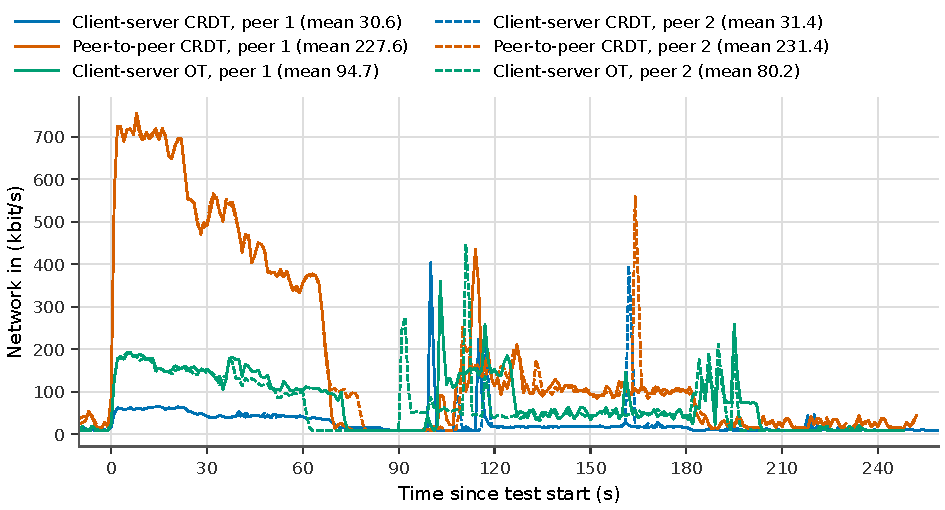
\includegraphics[width=\linewidth]{figures/s1-n8-peers-network-in}
 \caption{Incoming network data of the first and second clients, Scenario 1, $n = 8$.}
 \label{fig:2-23}
\end{figure}

The incoming traffic in Figure~\ref{fig:2-23} looks normal: the updates received are not very large. Figure~\ref{fig:2-25}, however, shows that the first client of the OT variant, which was disconnected at second 72 and reconnected at second 102, then sent a large amount of data for about 20 seconds. The same holds for the second client, disconnected at around second 60 and reconnected at second 90: right after a client reconnects, its outgoing traffic spikes. With many users in one document, disconnections and reconnections at similar times can make this variant unreliable.

\begin{figure}[htbp]
 \centering
 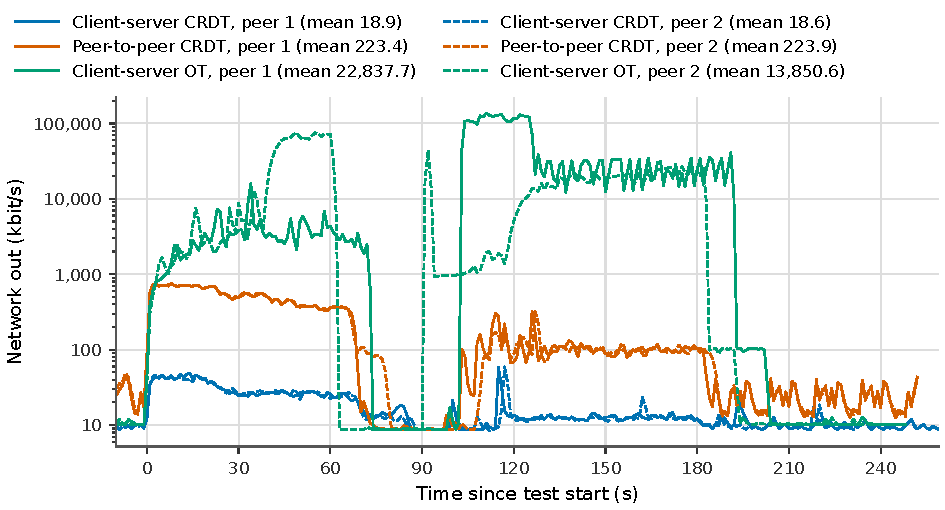
\includegraphics[width=\linewidth]{figures/s1-n8-peers-network-out}
 \caption[Outgoing network data of the first and second clients, Scenario 1, $n = 8$, on a logarithmic scale]{Outgoing network data of the first and second clients, Scenario 1, $n = 8$, on a logarithmic scale. The OT clients send up to a thousand times more than the CRDT clients, in bursts after their reconnection.}
 \label{fig:2-25}
\end{figure}

An update sent right after the connection is restored tends to be large, because it gathers the operations made while the client was offline. When it is sent, the server is also receiving updates from many other clients. The OT algorithm implemented here accepts an update only if the client's latest version matches the server's; otherwise, the server rejects the update and asks the client to pull first. Meanwhile, the backlog of large updates keeps being resent, and can saturate the server's bandwidth.

\begin{figure}[htbp]
 \centering
 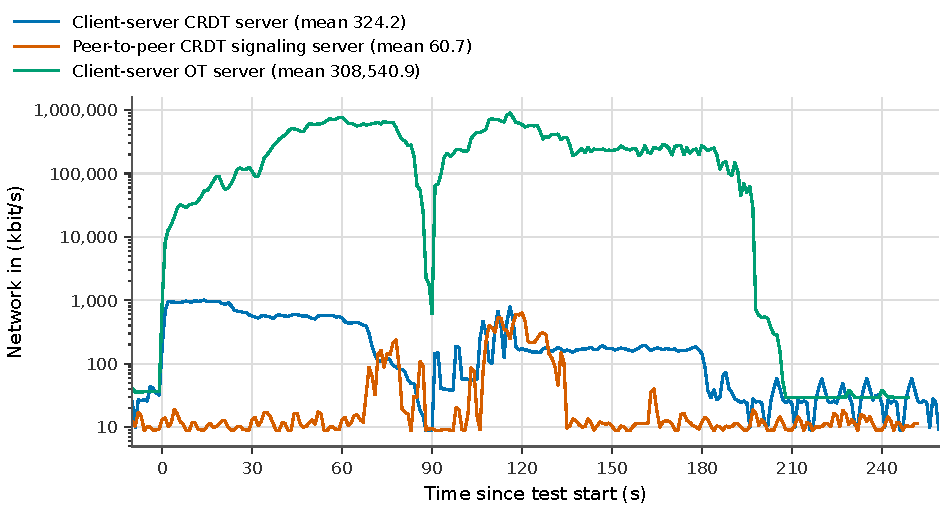
\includegraphics[width=\linewidth]{figures/s1-n8-server-network-in}
 \caption[Incoming network data of the servers, Scenario 1, $n = 8$, on a logarithmic scale]{Incoming network data of the servers, Scenario 1, $n = 8$, on a logarithmic scale. The signaling server of the peer-to-peer variant stays close to zero.}
 \label{fig:2-24}
\end{figure}

The traffic into the server of the client-server OT variant can exceed 800{,}000 kilobits per second, that is, 100 megabytes per second. Figure~\ref{fig:2-24} shows that its mean rate is about 950 times that of the client-server CRDT variant. The signaling server of the peer-to-peer CRDT variant, by contrast, shows almost no activity: it does not take part in the data exchange, because the peers communicate directly.

In Scenario 1, the CRDT variants are more reliable, because updates to the document can be merged in any order. Other likely factors are the implementation of the WebSocket provider and the compression and encoding Yjs uses. In the OT variant, updates also pile up because of large change operations, which take longer to arrive than the smaller updates of other clients. As a result, some clients have to pull repeatedly before they can push their own update, whenever their local version differs from the server's. This in turn affects two other aspects: scalability and responsiveness.

\section{The Scalability and Responsiveness Aspects}
\label{sec:5:latency}

The latency of the code editor was measured in Scenario 3, which, unlike Scenarios 1 and 2, has no disconnections. Each user measured the delay with which data from every other user arrived, recorded when the document data arrived, and these latencies were averaged over the $n$ users in the network. Table~\ref{tab:latency-3} gives the latency of nonlocal operations, that is, operations made by the other users in the network. The peer-to-peer CRDT variant has the lowest latency, although the gap between it and the client-server CRDT variant narrows as $n$ grows. The latency of the client-server OT variant is more than twice that of the client-server CRDT variant, nearly four times at $n = 8$, with spikes of about two seconds at $n = 8$.

\begin{table}[htbp]
 \centering
 \caption{Latency of nonlocal operations in Scenario 3 (shared code editor), in milliseconds.}
 \label{tab:latency-3}
 \begin{tabular}{@{}c rrr rrr rrr@{}}
 \toprule
 & \multicolumn{3}{c}{\textbf{Peer-to-peer CRDT}} & \multicolumn{3}{c}{\textbf{Client-server CRDT}} & \multicolumn{3}{c}{\textbf{Client-server OT}} \\
 \cmidrule(lr){2-4}\cmidrule(lr){5-7}\cmidrule(l){8-10}
 $n$ & Mean & Median & Max & Mean & Median & Max & Mean & Median & Max \\
 \midrule
 2 & 23.30 & 21 & 76  & 39.50 & 38 & 134 & 87.42  & 84  & 168 \\
 4 & 34.00 & 30 & 223 & 46.10 & 42 & 220 & 98.84  & 86  & 1{,}225 \\
 8 & 55.56 & 47 & 313 & 63.84 & 56 & 308 & 235.62 & 151 & 2{,}010 \\
 \bottomrule
 \end{tabular}
\end{table}

As for scalability: when all users are close to one another (in this experiment, all peers were in the same zone, in Indonesia), the peer-to-peer architecture performs better than the client-server one for the values of $n$ tested. The narrowing gap in Table~\ref{tab:latency-3} suggests, however, that the client-server CRDT variant may offer better responsiveness for larger $n$, or when the peers are farther apart.

Figure~\ref{fig:5:summary-latency} summarizes the latency measurements of Scenarios 3 and 4 against the number of users.

\begin{figure}[htbp]
 \centering
 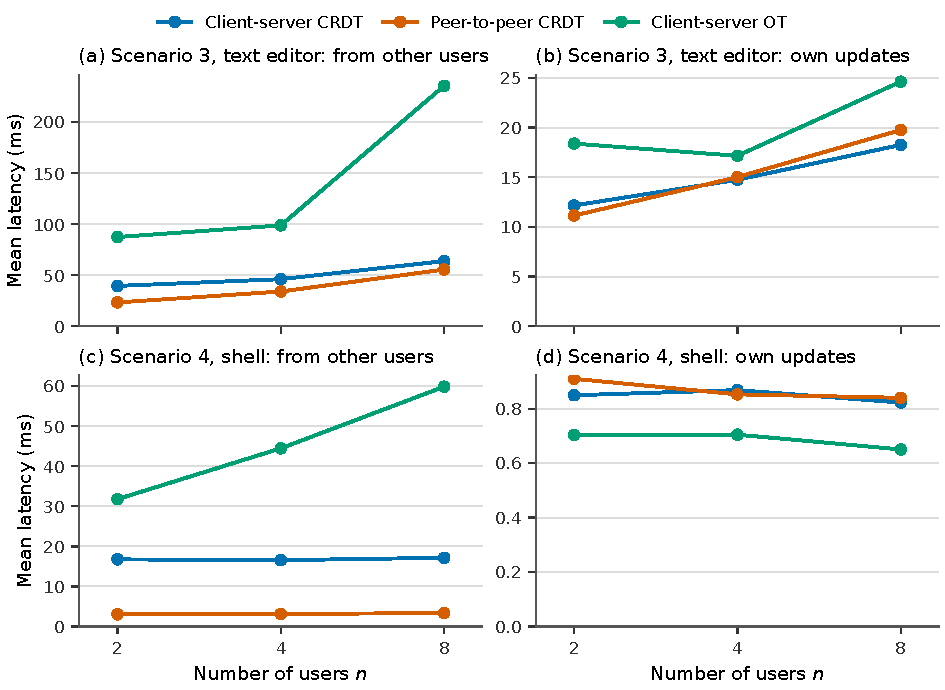
\includegraphics[width=\linewidth]{figures/summary-latency}
 \caption[Mean latency against the number of users $n$]{Mean latency against the number of users $n$. (a) and (c): updates from other users, as in Tables~\ref{tab:latency-3} and~\ref{tab:latency-4}; (b) and (d): the time to apply a user's own updates.}
 \label{fig:5:summary-latency}
\end{figure}

Part of the difference in latency may also come from the algorithm that keeps the replicas identical. To isolate it, the time to apply local changes was measured for each variant. A local operation here is one that a user makes on their own document: it is local-first and involves no network transmission. Figure~\ref{fig:12-5} shows only a small difference between the variants, about 5~ms on average, and small spikes, which can occur when characters are inserted or deleted at particular random positions. Note that the costs of CRDT and OT scale differently: the time complexity of OT depends on the number of concurrent operations, while that of a CRDT depends on the number of characters, that is, on the size of the document.

\begin{figure}[htbp]
 \centering
 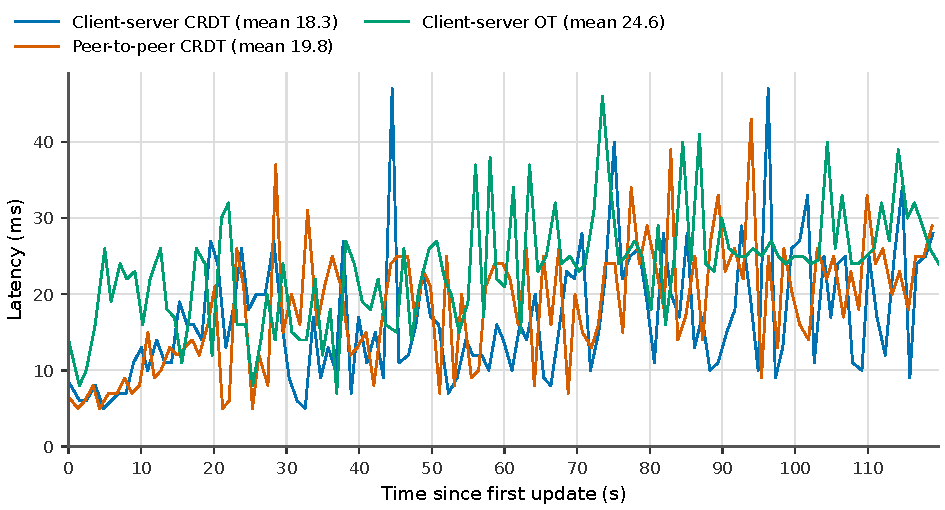
\includegraphics[width=\linewidth]{figures/s3-n8-latency-self}
 \caption{Time to apply local operations in the code editor, Scenario 3, $n = 8$.}
 \label{fig:12-5}
\end{figure}

The total latency is the time to apply local and nonlocal operations plus the network transmission time, which differs between the architectures. Figure~\ref{fig:7-5} shows larger differences between the variants, and several latency spikes over the course of Scenario 3. They have two likely causes: the time to resolve nonlocal operations, and the pile-up of updates illustrated in Figure~\ref{diagram:snowball}.

\begin{figure}[htbp]
 \centering
 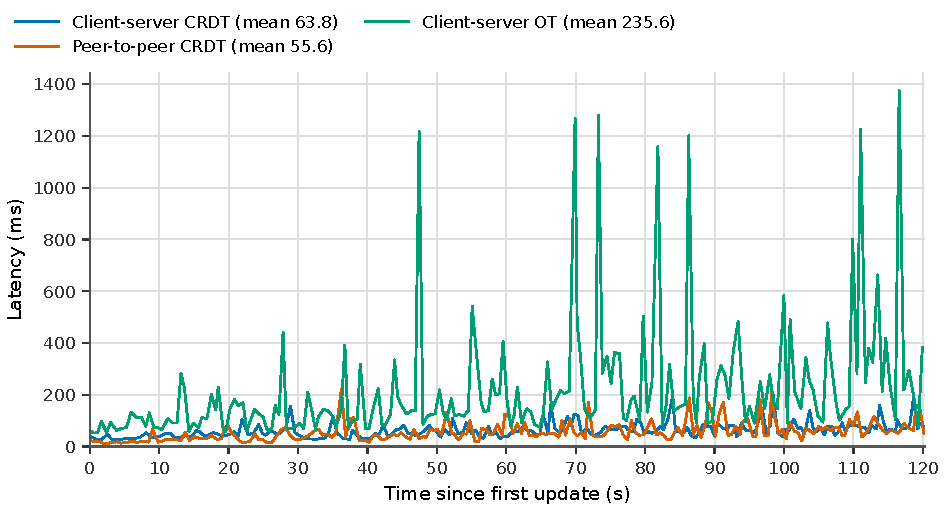
\includegraphics[width=\linewidth]{figures/s3-n8-latency-others}
 \caption{Latency of nonlocal operations in the code editor, Scenario 3, $n = 8$.}
 \label{fig:7-5}
\end{figure}

\begin{figure}[htbp]
 \centering
 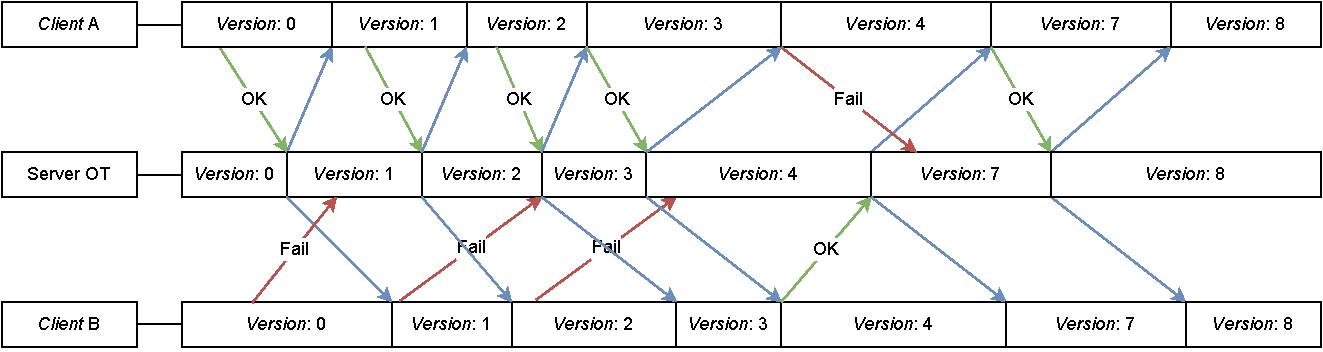
\includegraphics[width=\linewidth]{figures/ot-snowball}
 \caption[Updates piling up in the OT variant]{Updates piling up in the OT variant. Green arrows are pushes the server accepts, red arrows pushes it rejects because the client is behind, and blue arrows pulls. Client B's pushes keep failing while client A keeps getting its own in first.}
 \label{diagram:snowball}
\end{figure}

In the client-server OT architecture, the server does not accept an update from a client that does not have its latest version yet. Updates pile up when a client cannot get its data accepted, because its update keeps growing while other clients always get theirs in first. This holds back the updates of one or more clients, and makes the data the clients send, and the server receives, much larger than in the other variants.

In realistic use, this should not happen often, because users do not insert, delete and change characters as fast and as simultaneously as in Scenario 1. Repeated copy-and-paste operations could cause it, since they change many characters at once. Such operations, however, usually come with enough time between them for every client to update its replica before the next large change.

Scenario 4 tests the latency of the shared shell, which every user in the network can use at the same time; Table~\ref{tab:latency-4} summarizes it. In the code editor, applying a local operation took about 10 to 25~ms on average (Figure~\ref{fig:12-5}). The shell's data structure is a simple append-only list, so applying an operation takes almost no time in any variant, and the variants show no notable difference (Figure~\ref{fig:13-5}).

\begin{table}[htbp]
 \centering
 \caption{Latency of nonlocal operations in Scenario 4 (shared shell), in milliseconds.}
 \label{tab:latency-4}
 \begin{tabular}{@{}c rrr rrr rrr@{}}
 \toprule
 & \multicolumn{3}{c}{\textbf{Peer-to-peer CRDT}} & \multicolumn{3}{c}{\textbf{Client-server CRDT}} & \multicolumn{3}{c}{\textbf{Client-server OT}} \\
 \cmidrule(lr){2-4}\cmidrule(lr){5-7}\cmidrule(l){8-10}
 $n$ & Mean & Median & Max & Mean & Median & Max & Mean & Median & Max \\
 \midrule
 2 & 3.05 & 3 & 5  & 16.75 & 17 & 19 & 31.79 & 30    & 170 \\
 4 & 3.13 & 3 & 6  & 16.55 & 17 & 21 & 44.47 & 32    & 309 \\
 8 & 3.36 & 3 & 19 & 17.16 & 17 & 35 & 59.86 & 30.33 & 551 \\
 \bottomrule
 \end{tabular}
\end{table}

\begin{figure}[htbp]
 \centering
 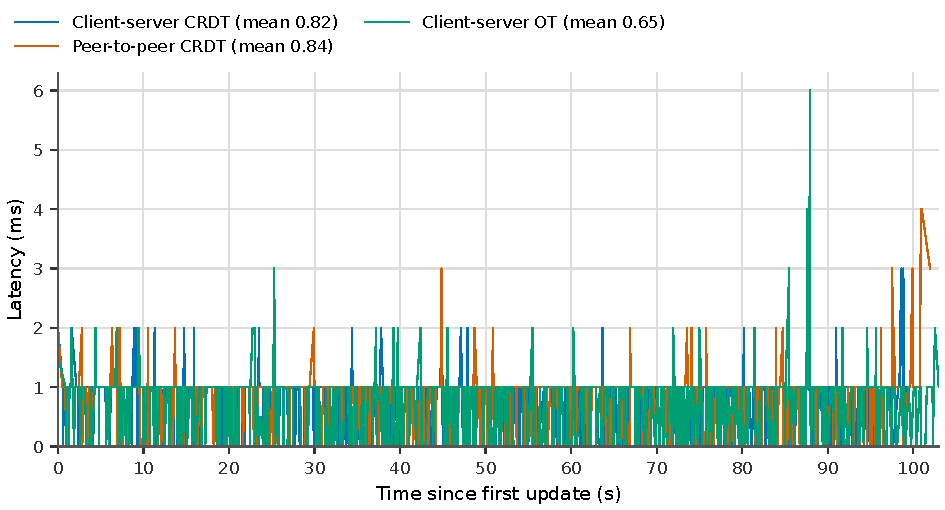
\includegraphics[width=\linewidth]{figures/s4-n8-latency-self}
 \caption{Time to apply local operations in the shared shell, Scenario 4, $n = 8$.}
 \label{fig:13-5}
\end{figure}

This is because appending to an append-only array takes amortized constant time. For the shell, scalability is therefore mainly a matter of how efficiently the data is transmitted, and shell updates in the OT variant suffer from the same problem as in Scenarios 1 and 3, as Figure~\ref{fig:9-5} shows.

Another reason why OT is slower than the client-server CRDT is its communication mechanism. The Yjs CRDT implementation encodes and decodes updates in a compact binary form, which makes transmitting large data faster, and a CRDT does not need updates to be applied in order. The OT variant, in contrast, uses the same update mechanism for the shell as for its code editor.

\begin{figure}[htbp]
 \centering
 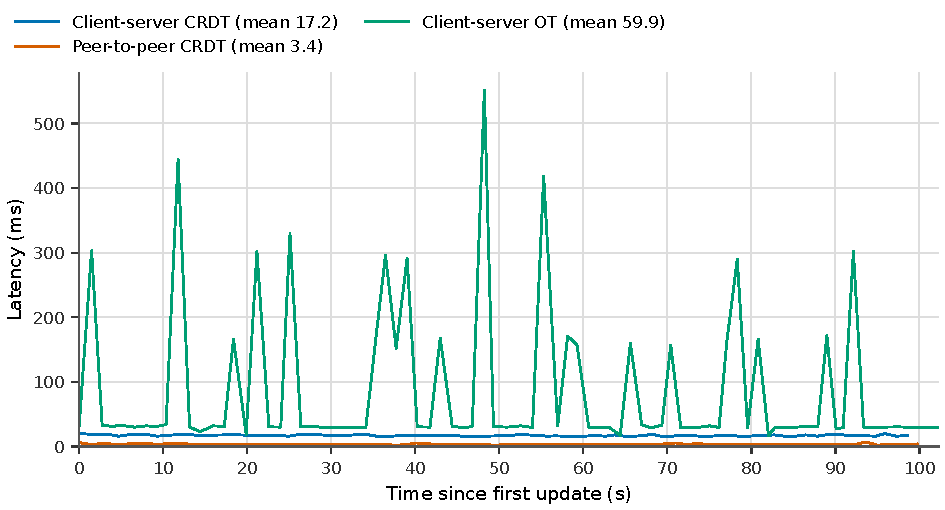
\includegraphics[width=\linewidth]{figures/s4-n8-latency-others}
 \caption{Latency of nonlocal operations in the shared shell, Scenario 4, $n = 8$.}
 \label{fig:9-5}
\end{figure}

In this experiment, the peers of the peer-to-peer variant were close to one another, in the same zone, and their latency was lower than in both client-server variants, whose traffic must pass through the server first. For $n \leq 8$, the peer-to-peer variant gives the best responsiveness of all the variants. For $n > 8$, or for peers farther apart, the client-server CRDT variant is expected to be worth considering as the better alternative.

Peers in the WebRTC-based variant may also be unable to connect to one another at all. A TURN relay server can then forward their traffic, at a latency that further experiments would have to measure. A better OT algorithm is also worth considering: in theory, its constant-time append operations could give the shell lower latency, by exploiting the append-only array and the fact that only the host of a shell forwards its interaction data. The CRDT data structure for the shell could likewise be modified to exploit these properties.

The system could also choose the best architecture automatically: peer-to-peer without a relay server, as in this experiment; peer-to-peer with a relay server, for peers that cannot connect directly over WebRTC; or client-server, when a network group has many clients. For latency, this choice could rest on a simple metric such as the ping between users, measured in the background. Other factors must be weighed as well, above all the lightweight aspect: how much processing, bandwidth and memory the server and the users must provide.

\section{The Lightweight Aspect}
\label{sec:5:lightweight}

This aspect describes how much computing resources each user and the server need. All RAM measurements were normalized to zero just before each test started, so that their growth can be compared. On the clients, the Electron application runs on Chromium, which has its own garbage collection and caching~\citep{chromium}, so memory is more meaningfully measured relative to its size just before the test. At the start, each server uses relatively little RAM, under 20~MiB, while each client starts at about 200~MiB, because the Electron framework runs a Chromium web browser for its front end.

\begin{table}[htbp]
 \centering
 \caption[Mean resource usage of the client application in Scenario 1]{Mean resource usage of the client application in Scenario 1. CPU in percent of one vCPU, RAM growth in MiB, network rates in kbit/s. Each value is the mean of the first two clients.}
 \label{tab:resource-client-1}
 \begin{tabular}{@{}llrrr@{}}
 \toprule
 \textbf{Variant} & \textbf{Metric} & $n = 2$ & $n = 4$ & $n = 8$ \\
 \midrule
 Peer-to-peer CRDT & CPU     & 39.20     & 60.14     & 62.29 \\
                   & RAM     & 16.58     & 19.24     & 21.30 \\
                   & Net in  & 28.52     & 96.17     & 229.48 \\
                   & Net out & 28.04  & 93.98  & 223.63 \\
 \midrule
 Client-server CRDT & CPU     & 33.96    & 57.39     & 56.89 \\
                    & RAM     & 14.93    & 19.13     & 20.95 \\
                    & Net in  & 19.47    & 27.69     & 30.97 \\
                    & Net out & 19.76 & 21.21  & 18.73 \\
 \midrule
 Client-server OT & CPU     & 47.79       & 73.29       & 65.26 \\
                  & RAM     & 25.95       & 31.17       & 36.34 \\
                  & Net in  & 62.24       & 99.81       & 87.42 \\
                  & Net out & 12{,}962.05 & 28{,}872.47 & 18{,}344.15 \\
 \bottomrule
 \end{tabular}
\end{table}

In Table~\ref{tab:resource-client-1}, 100\% CPU utilization means that the application fully uses one vCPU core. RAM usage and incoming data of the peer-to-peer CRDT variant grow the most with $n$ (Figure~\ref{fig:5:summary-clients}): the more peers there are in the network, the more replicas each peer must keep in sync, because the signaling server of this variant plays no part in transmitting CRDT data, and every peer exchanges updates with every other peer itself. All the data a CRDT client receives can be used immediately, with no rejected updates as in the OT variant. In terms of outgoing data, the CRDT variants therefore meet the lightweight aspect much better than the OT variant.

\begin{figure}[htbp]
 \centering
 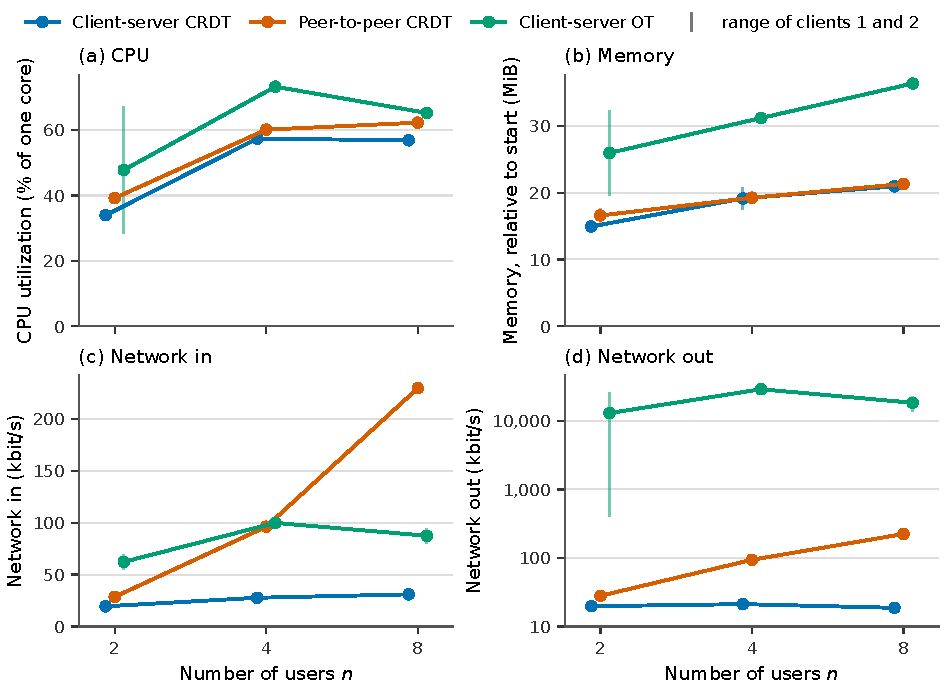
\includegraphics[width=\linewidth]{figures/summary-s1-clients}
 \caption[Mean resource usage of the client application in Scenario 1 against the number of users $n$]{Mean resource usage of the client application in Scenario 1 against the number of users $n$ (Table~\ref{tab:resource-client-1}). Each point is the mean of the first two clients; the thin bars span the two clients' own values. Network out is on a logarithmic scale.}
 \label{fig:5:summary-clients}
\end{figure}

Overall, the client-server CRDT variant is the lightest on the clients. In terms of CPU, on test machines with two vCPU cores (a maximum utilization of 200\%), every variant in Scenario 1 with $n \geq 4$ uses on average only about a third of the CPU, as Figure~\ref{fig:2-19} shows. These numbers should be read with the caveat that Scenario 1 is a much heavier load than normal use is expected to be. The operating system also decides which processes to prioritize, in memory and in CPU, while the application runs, so resource usage may be higher or lower depending on other activity on the machine.

\begin{figure}[htbp]
 \centering
 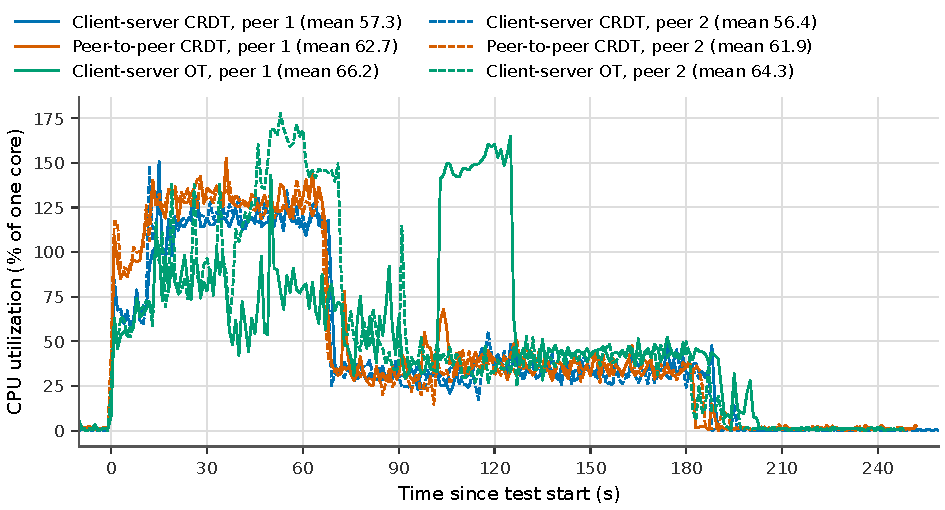
\includegraphics[width=\linewidth]{figures/s1-n8-peers-cpu}
 \caption{CPU utilization of the first and second clients, Scenario 1, $n = 8$.}
 \label{fig:2-19}
\end{figure}

\begin{figure}[htbp]
 \centering
 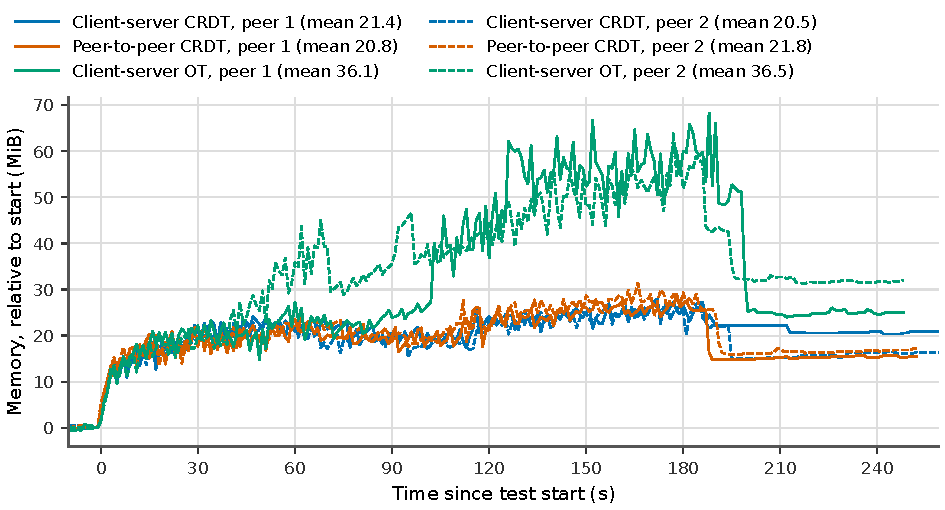
\includegraphics[width=\linewidth]{figures/s1-n8-peers-memory}
 \caption{Memory growth of the first and second clients, Scenario 1, $n = 8$.}
 \label{fig:2-21}
\end{figure}

Before normalization, memory usage starts at about 200~MiB on average, and then grows as Figure~\ref{fig:2-21} shows. Both CRDT variants grow less than the OT variant. Every variant, however, uses little memory compared with the capacity of the test machine, about 15\%. As long as the application does not load the machine to the point of disrupting the user's work, every variant of PeerToCP meets the lightweight aspect in terms of CPU and RAM.

\begin{table}[htbp]
 \centering
 \caption[Mean resource usage of the servers in Scenario 1]{Mean resource usage of the servers in Scenario 1, in the same units as Table~\ref{tab:resource-client-1}. For the peer-to-peer variant, the server is the signaling server.}
 \label{tab:resource-server-1}
 \begin{tabular}{@{}llrrr@{}}
 \toprule
 \textbf{Variant} & \textbf{Metric} & $n = 2$ & $n = 4$ & $n = 8$ \\
 \midrule
 Peer-to-peer CRDT & CPU     & 0.01     & 0.02     & 0.10 \\
                   & RAM     & 0.67     & $-$0.03  & 0.40 \\
                   & Net in  & 10.72    & 14.81    & 60.72 \\
                   & Net out & 10.24 & 15.79 & 83.11 \\
 \midrule
 Client-server CRDT & CPU     & 0.93     & 1.29      & 1.68 \\
                    & RAM     & 5.01     & 6.83      & 9.54 \\
                    & Net in  & 73.26    & 176.64    & 324.19 \\
                    & Net out & 71.79 & 193.90 & 391.66 \\
 \midrule
 Client-server OT & CPU     & 4.85        & 14.18       & 24.33 \\
                  & RAM     & 30.92       & 41.88       & 69.99 \\
                  & Net in  & 52{,}318.08    & 167{,}768.04   & 308{,}540.87 \\
                  & Net out & 26{,}494.76 & 84{,}932.31 & 156{,}178.28 \\
 \bottomrule
 \end{tabular}
\end{table}

Resource usage on the server is the other half of the lightweight aspect (Table~\ref{tab:resource-server-1}). The WebRTC signaling server of the peer-to-peer CRDT variant used minimal RAM and CPU. In the client-server architectures the server does much more: besides maintaining the connections of the clients in a network group, it keeps their replicas consistent. The server of the client-server CRDT variant sends and receives 1.4 to 2.6 times as much data as a single peer in the peer-to-peer variant.

\begin{figure}[htbp]
 \centering
 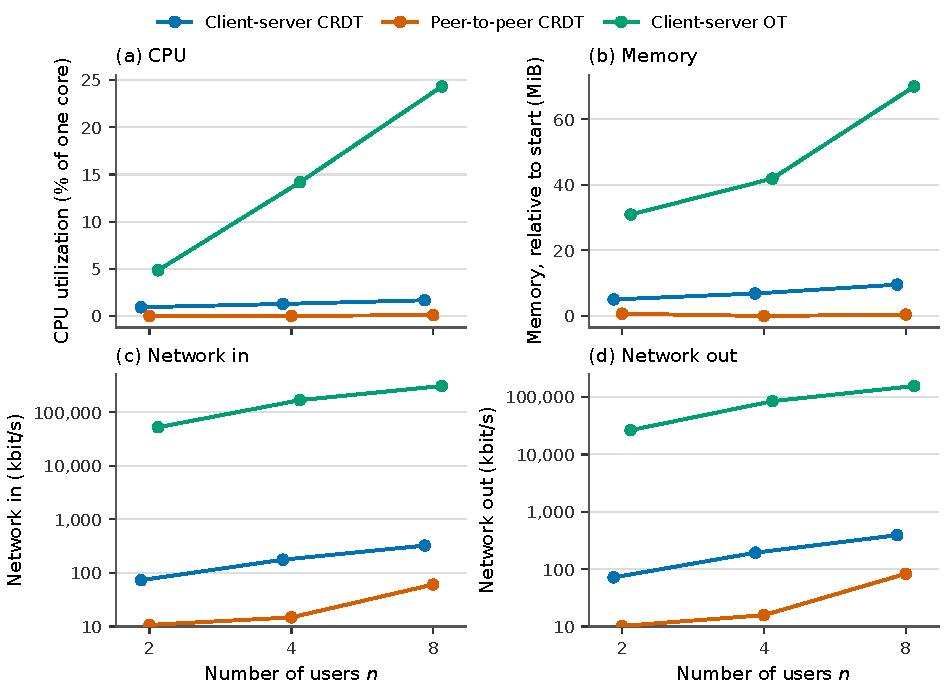
\includegraphics[width=\linewidth]{figures/summary-s1-server}
 \caption[Mean resource usage of the servers in Scenario 1 against the number of users $n$]{Mean resource usage of the servers in Scenario 1 against the number of users $n$ (Table~\ref{tab:resource-server-1}). For the peer-to-peer variant, the server is the signaling server. Network in and out are on logarithmic scales.}
 \label{fig:5:summary-server}
\end{figure}

\begin{figure}[htbp]
 \centering
 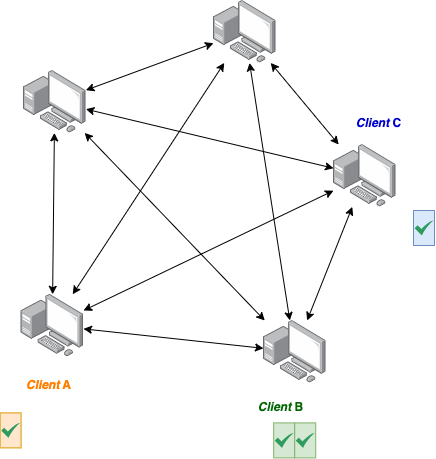
\includegraphics[width=4.08cm]{figures/crdt-sync-1}\hfill
 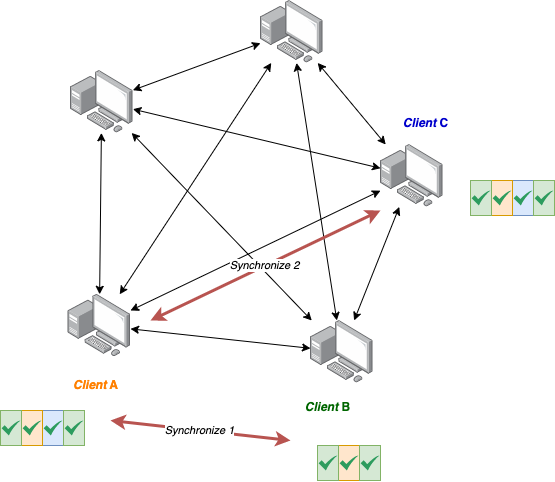
\includegraphics[width=4.8cm]{figures/crdt-sync-2}\hfill
 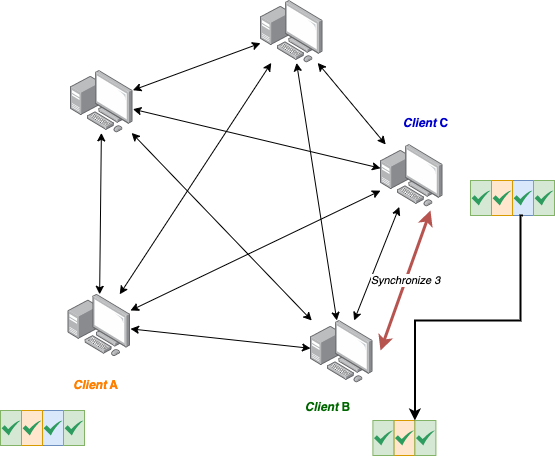
\includegraphics[width=4.8cm]{figures/crdt-sync-3}
 \caption[Synchronization in the peer-to-peer CRDT variant]{Synchronization in the peer-to-peer CRDT variant. Client A synchronizes with client B, then with client C; when B and C then synchronize, C only sends what B has not already received from A.}
 \label{fig:syncCRDT}
\end{figure}

The Yjs CRDT keeps a logical timestamp in the form of a state vector, which records the version of every user in the network. When two users synchronize, only the difference between their versions, derived from their state vectors, is sent; if the documents differ too much, the whole document may be sent instead, which can be smaller. Changes derived from the state vector are commutative and idempotent: the same change can be applied repeatedly and in any order without affecting the convergence of the document. Because of these properties, the data sent to each client does not depend on the number of operations performed, but on the size of the changes at the time of synchronization.

In Figure~\ref{fig:syncCRDT}, if client A first synchronizes with client B, then client A synchronizes with client C, and then client B synchronizes with client C, client C only needs to send B what B has not already received from client A. And if an object in the data structure is deleted before it has been synchronized, its content never needs to be sent at all. These are among the Yjs optimizations that reduce the total bandwidth between users in the CRDT variants.

Some reference implementations add an external database to store documents in the client-server architecture, so that a network group can hold more documents. None of the variants here uses a third-party database; each keeps only simple built-in data structures on the server. In the peer-to-peer architecture, documents can instead be persisted in the local storage of each peer.

\begin{figure}[htbp]
 \centering
 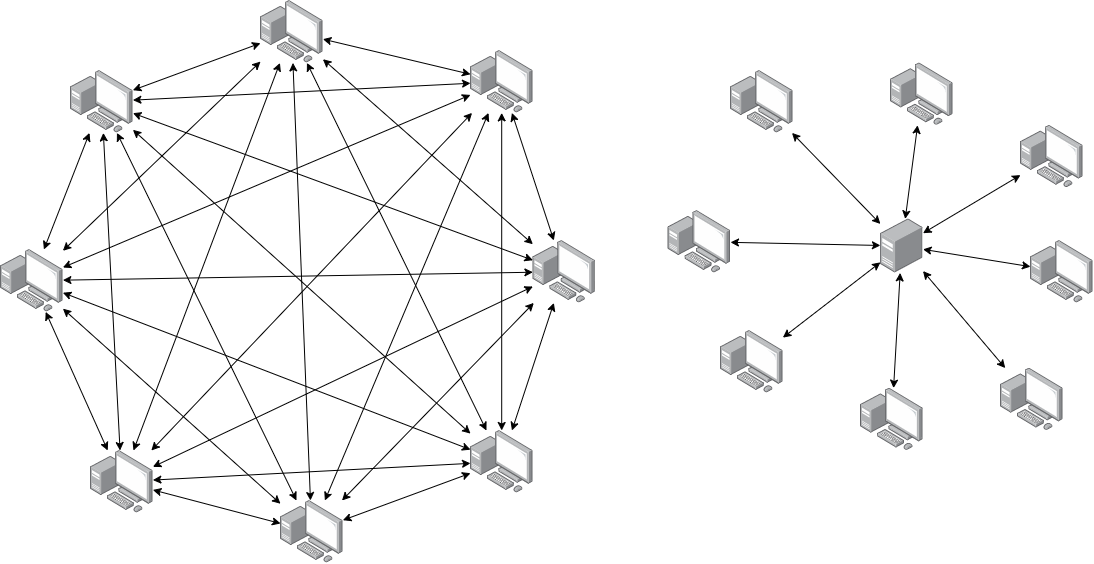
\includegraphics[width=11cm]{figures/mesh-vs-star}
 \caption{Connections in a peer-to-peer full mesh (left) and in a client-server star (right), for eight users.}
 \label{fig:compare}
\end{figure}

The price of the client-server CRDT variant's light traffic on the clients is heavier traffic on the server. In the peer-to-peer variant, on the other hand, the number of data channel connections grows quadratically with the number of users (Figure~\ref{fig:compare}), so the total traffic each peer must handle grows faster with the size of the network group. The OT variant, given its conflict-resolution protocol, has by far the largest network load of all the variants, which also drives up its CPU and RAM usage. From the lightweight perspective, the client-server OT variant is not preferred, and its data transmission protocol needs to be revisited and optimized. More sophisticated and better-optimized OT algorithms also deserve further study, so that intensive editing such as in Scenario 1 can be handled.
